% -- LICENSE BEGIN --
%
% Copyright (c) 2015-2018, Lawrence Livermore National Security, LLC.
%
% Produced at the Lawrence Livermore National Laboratory
%
% Written by
%   Michael Bentley (mikebentley15@gmail.com),
%   Geof Sawaya (fredricflinstone@gmail.com),
%   and Ian Briggs (ian.briggs@utah.edu)
% under the direction of
%   Ganesh Gopalakrishnan
%   and Dong H. Ahn.
%
% LLNL-CODE-743137
%
% All rights reserved.
%
% This file is part of FLiT. For details, see
%   https://pruners.github.io/flit
% Please also read
%   https://github.com/PRUNERS/FLiT/blob/master/LICENSE
%
% Redistribution and use in source and binary forms, with or
% without modification, are permitted provided that the following
% conditions are met:
%
% - Redistributions of source code must retain the above copyright
%   notice, this list of conditions and the disclaimer below.
%
% - Redistributions in binary form must reproduce the above
%   copyright notice, this list of conditions and the disclaimer
%   (as noted below) in the documentation and/or other materials
%   provided with the distribution.
%
% - Neither the name of the LLNS/LLNL nor the names of its
%   contributors may be used to endorse or promote products derived
%   from this software without specific prior written permission.
%
% THIS SOFTWARE IS PROVIDED BY THE COPYRIGHT HOLDERS AND
% CONTRIBUTORS "AS IS" AND ANY EXPRESS OR IMPLIED WARRANTIES,
% INCLUDING, BUT NOT LIMITED TO, THE IMPLIED WARRANTIES OF
% MERCHANTABILITY AND FITNESS FOR A PARTICULAR PURPOSE ARE
% DISCLAIMED. IN NO EVENT SHALL LAWRENCE LIVERMORE NATIONAL
% SECURITY, LLC, THE U.S. DEPARTMENT OF ENERGY OR CONTRIBUTORS BE
% LIABLE FOR ANY DIRECT, INDIRECT, INCIDENTAL, SPECIAL,
% EXEMPLARY, OR CONSEQUENTIAL DAMAGES (INCLUDING, BUT NOT LIMITED
% TO, PROCUREMENT OF SUBSTITUTE GOODS OR SERVICES; LOSS OF USE,
% DATA, OR PROFITS; OR BUSINESS INTERRUPTION) HOWEVER CAUSED AND
% ON ANY THEORY OF LIABILITY, WHETHER IN CONTRACT, STRICT
% LIABILITY, OR TORT (INCLUDING NEGLIGENCE OR OTHERWISE) ARISING
% IN ANY WAY OUT OF THE USE OF THIS SOFTWARE, EVEN IF ADVISED OF
% THE POSSIBILITY OF SUCH DAMAGE.
%
% Additional BSD Notice
%
% 1. This notice is required to be provided under our contract
%    with the U.S. Department of Energy (DOE). This work was
%    produced at Lawrence Livermore National Laboratory under
%    Contract No. DE-AC52-07NA27344 with the DOE.
%
% 2. Neither the United States Government nor Lawrence Livermore
%    National Security, LLC nor any of their employees, makes any
%    warranty, express or implied, or assumes any liability or
%    responsibility for the accuracy, completeness, or usefulness of
%    any information, apparatus, product, or process disclosed, or
%    represents that its use would not infringe privately-owned
%    rights.
%
% 3. Also, reference herein to any specific commercial products,
%    process, or services by trade name, trademark, manufacturer or
%    otherwise does not necessarily constitute or imply its
%    endorsement, recommendation, or favoring by the United States
%    Government or Lawrence Livermore National Security, LLC. The
%    views and opinions of authors expressed herein do not
%    necessarily state or reflect those of the United States
%    Government or Lawrence Livermore National Security, LLC, and
%    shall not be used for advertising or product endorsement
%    purposes.
%
% -- LICENSE END --

\documentclass[border=10pt]{standalone}
\usepackage{pgfplots}
\pgfplotsset{width=7cm, compat=1.8}
\usepackage{pgfplotstable}
\renewcommand*{\familydefault}{\sfdefault}
\usepackage{sfmath}
\usepackage{graphicx}

\begin{document}

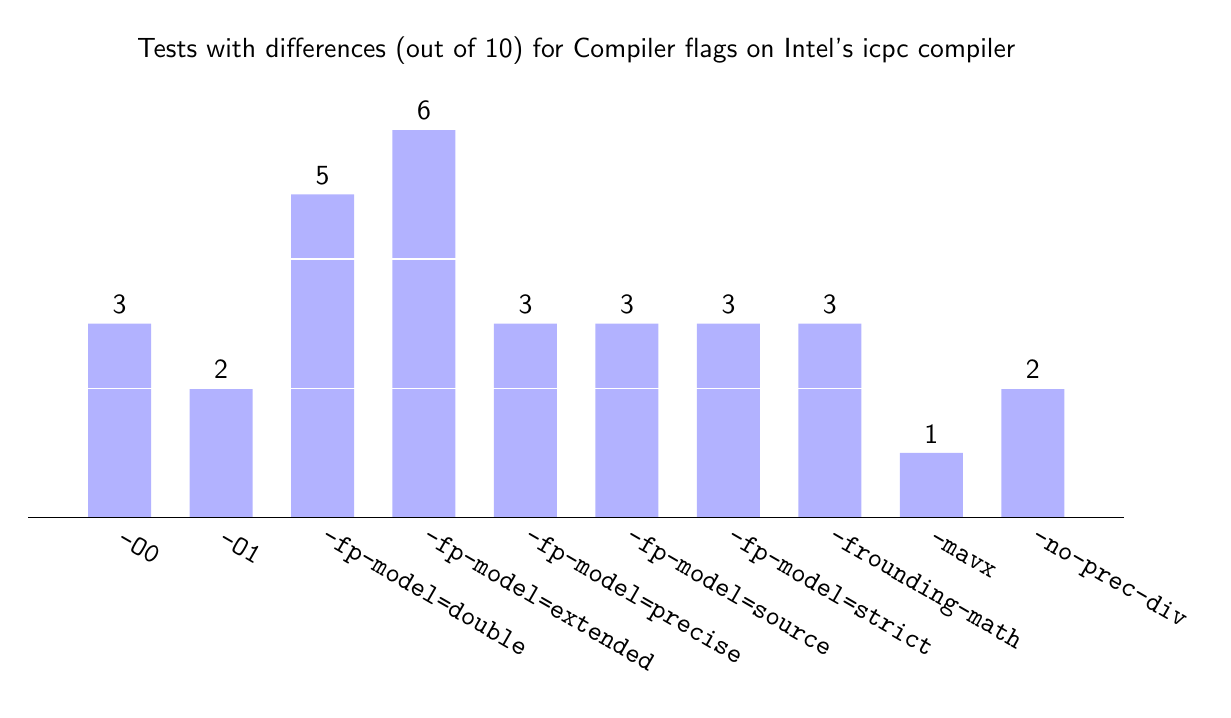
\begin{tikzpicture}
  \centering
  \begin{axis}[
    ybar,
    axis on top,
    title={Tests with differences (out of 10) for Compiler flags on Intel's icpc compiler},
    height=7cm,
    width=15.5cm,
    bar width=0.8cm,
    ymajorgrids,
    tick align=inside,
    major grid style={draw=white},
    ymin=0,
    axis x line*=bottom,
    axis y line*=right,
    y axis line style={opacity=0},
    yticklabel style={opacity=0},
    tickwidth=0pt,
    enlarge x limits=true,
    symbolic x coords={
      -O0,
      -O1,
      -fp-model=double,
      -fp-model=extended,
      -fp-model=precise,
      -fp-model=source,
      -fp-model=strict,
      -frounding-math,
      -mavx,
      -no-prec-div,
      },
    xtick=data,
    xticklabel style={ rotate=-30, anchor=west, yshift=-0.2cm , font=\ttfamily },
    nodes near coords={
      \pgfmathprintnumber[precision=0]{\pgfplotspointmeta}
      },
    ]
    \addplot [draw=none, fill=blue!30] coordinates {
      (-fp-model=extended, 6)
      (-fp-model=double,   5)
      (-fp-model=source,   3)
      (-fp-model=strict,   3)
      (-frounding-math,    3)
      (-O0,                3)
      (-fp-model=precise,  3)
      (-no-prec-div,       2)
      (-O1,                2)
      (-mavx,              1)
      };
  \end{axis}
  This is compared with having no command-line arguments at all (except
  -mlong-double-80 which was used for all runs)
\end{tikzpicture}



%\begin{tikzpicture}
%  \centering
%  \begin{axis}[
%    ybar,
%    axis on top,
%    title={Cumulative Progress of Works},
%    height=7cm,
%    width=15.5cm,
%    bar width=0.4cm,
%    ymajorgrids,
%    tick align=inside,
%    major grid style={draw=white},
%    enlarge y limits={value=.1,upper},
%    ymin=0,
%    ymax=100,
%    axis x line*=bottom,
%    axis y line*=right,
%    y axis line style={opacity=0},
%    tickwidth=0pt,
%    enlarge x limits=true,
%    legend style={
%      at={(0.5,-0.2)},
%      anchor=north,
%      legend columns=-1,
%      /tikz/every even column/.append style={column sep=0.5cm}
%      },
%    ylabel={Percentage (\%)},
%    symbolic x coords={
%      Sep-11,
%      Oct-11,
%      Nov-11,
%      Dec-11,
%      Jan-12,
%      Feb-12,
%      Mar-12,
%      Apr-12,
%      },
%    xtick=data,
%    nodes near coords={
%      \pgfmathprintnumber[precision=0]{\pgfplotspointmeta}
%      },
%    ]
%    \addplot [draw=none, fill=blue!30] coordinates {
%      (Sep-11, 75.4064)
%      (Oct-11, 72.7961)
%      (Nov-11, 94.4597)
%      (Dec-11, 66.6786)
%      (Jan-12, 67.5600)
%      (Feb-12, 88.2339)
%      (Mar-12, 78.6138)
%      (Apr-12, 58.9129)
%      };
%   \addplot [draw=none,fill=red!30] coordinates {
%      (Sep-11, 75.4064)
%      (Oct-11, 89.7961)
%      (Nov-11, 94.4597)
%      (Dec-11, 76.6786)
%      (Jan-12, 77.5600)
%      (Feb-12, 78.2339)
%      (Mar-12, 88.6138)
%      (Apr-12, 78.9129) };
%   \addplot [draw=none, fill=green!30] coordinates {
%      (Sep-11, 75.4064)
%      (Oct-11, 89.7961)
%      (Nov-11, 94.4597)
%      (Dec-11, 76.6786)
%      (Jan-12, 77.5600)
%      (Feb-12, 78.2339)
%      (Mar-12, 88.6138)
%      (Apr-12, 78.9129) };
%
%    \legend{First Fix,Second Fix,Third Fix}
%  \end{axis}
%\end{tikzpicture}


\end{document}
